%%%%%%%%%%%%%%%%%%%%%%%%%%%%%%%%%%%%%%%%%%%%%%%%%%%%%%%%%%%%%%%%%%%%%%%%%%%%%
%%%                            Navigator                                  %%%
%%%%%%%%%%%%%%%%%%%%%%%%%%%%%%%%%%%%%%%%%%%%%%%%%%%%%%%%%%%%%%%%%%%%%%%%%%%%%
\subsubsection{Navigator}
\label{sec:uinavigator}
\index{NAVIGATOR@\NAVIGATOR}
The navigator is used to display datapool-structures like a
tree using folders and subfolders. \\

The routine used to find the pictures to use is described
in section \nameref{sec:uinavigatorPixmaps} page \pageref{sec:uinavigatorPixmaps}. \\

\begin{figure}[H]\label{fig:navigator}
   \begin{center}
      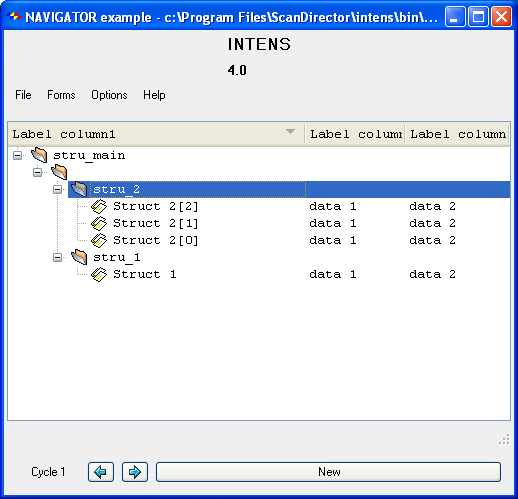
\includegraphics[width=0.6\linewidth]{grab_navigator}
   \end{center}
\caption{example of a Navigator tree}
\end{figure}

\input{diagrams/ui_navigator_type_option}

\index{ICONVIEW@\ICONVIEW!navigator type}
\index{DIAGRAM@\DIAGRAM!navigator type}
\begin{tabularx}{\textwidth}{l|X}
Navigator type & description \\
\hline
\ICONVIEW     & Show as icons. \newline
                See section \nameref{sec:uinavigatorIconView} page \pageref{sec:uinavigatorIconView}. \\
\DIAGRAM      & Create a diagram to place, move and connect items. \newline
                See section \nameref{sec:uinavigatorDiagram} page \pageref{sec:uinavigatorDiagram}. \\
\end{tabularx}

\newpage
\input{diagrams/ui_navigator_list}

\index{NAVIGATOR@\NAVIGATOR!options}
The options are mandatory when using structures that do not have a
   field named {\bfseries name} (examples page \pageref{sec:uinavigatorexamples}).
   The \TAG{} identifier must be declared (see \COL{}
   declaration page \pageref{sec:uinavigatoroptions}) to define the columns
   that should be displayed. \\

\input{diagrams/ui_navigator_option_list}
\label{sec:uinavigatoroptions}

\index{SIZE@\SIZE!navigator option}
\index{EXPAND@\EXPAND!navigator option}
\index{COL@\COL!navigator option}
\index{TOOLTIP@\TOOLTIP!navigator option}
\index{MULTIPLE\_SELECTION@\MULTIPLESELECTION!navigator option}
\index{COMPARE@\COMPARE!navigator option}
\index{NAVIGATOR@\NAVIGATOR!SIZE}
\index{NAVIGATOR@\NAVIGATOR!EXPAND}
\index{NAVIGATOR@\NAVIGATOR!COL}
\index{NAVIGATOR@\NAVIGATOR!TOOLTIP}
\index{NAVIGATOR@\NAVIGATOR!MULTIPLE\_SELECTION}
\index{NAVIGATOR@\NAVIGATOR!COMPARE}
\begin{tabularx}{\textwidth}{l|X}
Navigator options  & description \\
\hline
\SIZE              & Size of navigator window. \\
\EXPAND            & TODO. \\
\COL               & Columns declarations. \\
\TOOLTIP           & the value of the referenced structure field is shown as the
                     tooltip of this row \\
\MULTIPLESELECTION & enable the selection of multiple rows
                     (see function statement \GETSELECTION{} on page \pageref{dia:guimorestatement}).\\
\COMPARE           & This navigator is used to display a compare result
                     (see function statement \COMPARE{} on page \pageref{dia:datastatement}).\\
\end{tabularx}

\input{diagrams/ui_navigator_col_list}
\index{TAG@\TAG!navigator}
\index{PIXMAP@\PIXMAP!navigator col option}
\index{SORT@\SORT!navigator col option}

\begin{tabularx}{\textwidth}{l|X}
Columns declaration     & description \\
\hline
\verb+string+           & colunm title \\
\verb+ID TAG+           & references a structure field previously declared in
                           datapool section (see section \nameref{dia:dataitemoptions}
                           on page \pageref{dia:dataitemoptions}). \\
\verb+ui field attributes+ & defines, how fields are displayed
                          {\bfseries(*scale :width :precision :tsep)}.
                          See section \nameref{dia:uifieldattributes} page \pageref{dia:uifieldattributes}. \\
\PIXMAP                 & TODO \\
\SORT                   & The navigator rows are sorted using this column.
                          You can select an other column using the mouse. \\
\end{tabularx}

\newpage
\input{diagrams/ui_navigator_root_list}
\index{root-list}

\index{NAVIGATOR@\NAVIGATOR!root list}
\begin{tabularx}{\textwidth}{l|X}
Root list                   & description \\
\hline
\verb+structure identifier+ & references a structure previously
                  declared in datapool section.
                           (\nameref{sec:dpstruct} page \pageref{sec:dpstruct}) \\
\end{tabularx}

\input{diagrams/ui_navigator_root_option_list}
\index{root-list options}

\index{AUTOLEVEL@\AUTOLEVEL!navigator}
\index{HIDEEMPTYFOLDERS@\HIDEEMPTYFOLDERS!navigator}
\index{OPENLEVELS@\OPENLEVELS!navigator}
\index{FIRSTLEVEL@\FIRSTLEVEL!navigator}
\index{LASTLEVEL@\LASTLEVEL!navigator}
\index{NAVIGATOR@\NAVIGATOR!AUTOLEVEL}
\index{NAVIGATOR@\NAVIGATOR!HIDE\_EMPTY\_FOLDERS}
\index{NAVIGATOR@\NAVIGATOR!OPENLEVELS}
\index{NAVIGATOR@\NAVIGATOR!FIRSTLEVEL}
\index{NAVIGATOR@\NAVIGATOR!LASTLEVEL}
\begin{tabularx}{\textwidth}{l|X}
Root list options & description \\
\hline
\AUTOLEVEL        & Does not display any structure-identifiers at all. \\
\HIDEEMPTYFOLDERS & Does not display any structure-identifiers without entries. \\
\OPENLEVELS       & Displays open folders beginnig in tree-level 'integer'. \\
\FIRSTLEVEL       & Does not display structure-identifiers before tree-level 'integer'. \\
\LASTLEVEL        & Stops display after tree-level 'integer'. \\
\end{tabularx}

\newpage
\index{NAVIGATOR@\NAVIGATOR!structure definition}
\label{sec:uinavigatorexamples}
Example of structure definition with name items: \\


\begin{boxedminipage}[t]{\linewidth}
\begin{alltt}
DATAPOOL
  STRUCT
    STRU\_1 \{
      STRING \{EDITABLE\}
        {\bfseries name},
        data_item_1,
        data_item_2
      ;
    \};
  STRUCT
    STRU_2 \{
      STRING \{EDITABLE\}
        {\bfseries name},
        data_item_1,
        data_item_2
      ;
    \};
  STRUCT
    STRU_MAIN \{
      STRING \{EDITABLE\}
        {\bfseries name};
      STRU_1
        stru_1;
      STRU_2
        stru_2;
    \};
  STRU_MAIN
    stru_main
  ;
END DATAPOOL;
\end{alltt}
\end{boxedminipage}

\vspace{0.5cm}

Example of corresponding navigator definition: \\

\begin{boxedminipage}[t]{\linewidth}
\begin{alltt}
UI_MANAGER
  NAVIGATOR
    navigator_identifier
    (
      stru_main[*]
    )
  ;
END UI_MANAGER;
\end{alltt}
\end{boxedminipage}


\newpage
\index{NAVIGATOR@\NAVIGATOR!structure definition}
Example of structure definition without name items: \\


\begin{boxedminipage}[t]{\linewidth}
\begin{alltt}
DATAPOOL
  STRUCT
    STRU\_1 \{
      STRING \{EDITABLE\}
        {\bfseries noname}   \{TAG = (tag_col_1)\},
        data_item_1    \{TAG = (tag_col_2)\},
        data_item_2    \{TAG = (tag_col_3)\}
      ;
    \};
  STRUCT
    STRU_2 \{
      STRING \{EDITABLE\}
        {\bfseries noname}   \{TAG = (tag_col_1)\},
        data_item_1    \{TAG = (tag_col_2)\},
        data_item_2    \{TAG = (tag_col_3)\}
      ;
    \};
  STRUCT
    STRU_MAIN \{
      STRING \{EDITABLE\}
        {\bfseries noname}   \{TAG = (tag_col_1)\};
      STRU_1
        stru_1;
      STRU_2
        stru_2;
    \};
  STRU_MAIN
    stru_main
  ;
END DATAPOOL;
\end{alltt}
\end{boxedminipage}

\vspace{0.5cm}

Example of corresponding navigator definition: \\

\begin{boxedminipage}[t]{\linewidth}
\begin{alltt}
UI_MANAGER
  NAVIGATOR
    navigator_identifier
    \{ COL ("Label column1" {\bfseries tag\_col\_1}:20,
            "Label column2" {\bfseries tag\_col\_2}:10,
            "Label column3" {\bfseries tag\_col\_3}:10)
    \}
    (
      stru_main[*]
    )
  ;
END UI_MANAGER;
\end{alltt}
\end{boxedminipage}


\newpage
\label{navigatordragndrop}
\index{NAVIGATOR@\NAVIGATOR!drag and drop}
\index{drag and drop (navigator)}
\index{SOURCE@\SOURCE!function statement!navigator example}
\index{FUNCTIONS@\FUNCTIONS!\INIT!example}
\index{REASON_ACTIVATE@\REASONACTIVATE!function exression!navigator example}
\index{REASON_DROP@\REASONDROP!function exression!navigator example}
\index{REASON_SELECT@\REASONSELECT!function exression!navigator example}
Example of functions to encounter events like {\bfseries select} or {\bfseries drag and drop}:

\begin{boxedminipage}[t]{\linewidth}
\begin{alltt}
DESCRIPTION "Implementing menu and drag'n'drop functions";
DATAPOOL
  STRUCT Motor \{
    INTEGER   id;
    REAL      nom_power        \{TAG=Tpower\};
    STRING    id_manuf         \{TAG=Tmanuf\};
    STRING    model            \{TAG=Tname\};
    REAL      nom_voltage;
    REAL      nom_frequency;
  \};
   Motor motors                \{FUNC={\bfseries select\_motor}\};
END DATAPOOL;
FUNCTIONS
  FUNC INIT {
    motors[0].nom_power = 2.5;
    motors[0].id_manuf = "ABB";
    motors[0].model="QU 132";
    motors[0].nom_voltage=400;
    motors[0].nom_frequency=50;
    motors[1].nom_power = 7.5;
    .
    .
  };
  FUNC {\bfseries select\_motor} \{
    IF( REASON_SELECT )\{
      SET_MSG( THIS.model, " selected" ); \}
    ELSE IF( REASON_UNSELECT )\{
      SET_MSG( THIS.model, " unselected" ); \}
    ELSE IF( REASON_ACTIVATE )\{
      SET_MSG( THIS.model, " activated" ); \}
    ELSE IF( REASON_DROP )\{
      SET_MSG( SOURCE.model, " dropping to ", THIS.model ); \}
  \};
  FUNC DeleteThisMotor_func \{
    PRINT "Delete: ", THIS.model, EOLN;
  \};
  FUNC MoveThisMotor_func \{
    PRINT "Move: ", THIS.model, EOLN;
  \};
END FUNCTIONS;
UI_MANAGER
  NAVIGATOR
    motornav \{ COL( "" Tname:20
                  , "Manuf." Tmanuf:12
                  , "Output [kW]" Tpower:15 )\} (
      motors[*] = "Motors" );

  MENU Motor (
    FUNC DeleteThisMotor_func = "Delete This Motor"
   ,FUNC MoveThisMotor_func = "Move This Motor"
  );
END UI_MANAGER;
\end{alltt}
\end{boxedminipage}



\label{navigatormenu}
\index{NAVIGATOR@\NAVIGATOR!menu}
\index{MENU@\MENU!UI\_MANAGER!NAVIGATOR}
To add a popup \MENU{} to a navigator tree,
the menu identifier must be the same as the structure identifier:

\begin{boxedminipage}[t]{\linewidth}
\begin{alltt}
DESCRIPTION "Implementing menu and drag'n'drop functions";
DATAPOOL
  STRUCT Motor \{
    INTEGER   id;
    REAL      nom_power        \{TAG=Tpower\};
    STRING    id_manuf         \{TAG=Tmanuf\};
    STRING    model            \{TAG=Tname\};
    REAL      nom_voltage;
    REAL      nom_frequency;
  \};
  {\bfseries Motor} motors                 \{FUNC=select_motor\};
END DATAPOOL;
.
.
.
UI_MANAGER
  NAVIGATOR
    motornav \{ COL( "" Tname:20
                  , "Manuf." Tmanuf:12
                  , "Output [kW]" Tpower:15 )\} (
      motors[*] = "Motors" );

  MENU {\bfseries Motor} (
    FUNC DeleteThisMotor_func = "Delete This Motor"
   ,FUNC MoveThisMotor_func = "Move This Motor"
  );
END UI_MANAGER;
\end{alltt}
\end{boxedminipage}

\newpage
\subsubsection{Navigator IconView}
\label{sec:uinavigatorIconView}
This \NAVIGATOR{} type is used to show several elements
that can be dragged to a \DIAGRAM.

The \NAVIGATOR{} itself has one \COL{} with a \TAG{}.
The data item (parent in the example below) must have an attribute with that tag
(name in the example).
The \ICONVIEW{} shows all children of it that have an attribute with that tag
(parent.elements[*] with name in the example).

\begin{center}
  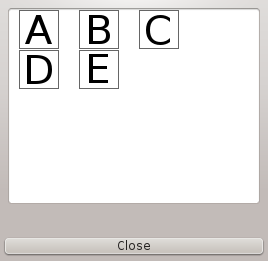
\includegraphics[width=0.3\linewidth]{examples/navigator/iconView}
\end{center}

\begin{boxedminipage}[t]{\linewidth}
\begin{alltt}
DATAPOOL
  STRUCT
    Elements \{
      STRING \{EDITABLE\}
        name \{ TAG=(nametag) \}
      , type
      ;
    \}
  ;
  STRUCT
    Parent \{
      STRING \{EDITABLE\}
        name \{ TAG=(nametag) \}
      ;
      Elements elements;
    \}
  ;
  Parent parent;
END DATAPOOL;

UI_MANAGER
  NAVIGATOR \{ ICONVIEW \}
    iconView_navigator
    \{ SIZE ( 200, 200 )
    , COL ("" nametag)
    , TOOLTIP(nametag)
    \}
    (
      parent \{ AUTOLEVEL \}
    )
  ;
  FORM
    iconView_form \{ HIDE_CYCLE \} (
      iconView_navigator
    )
  ;
END UI_MANAGER;

FUNCTIONS
  FUNC
    INIT \{
      parent.elements[0].name = "A";
      parent.elements[1].name = "B";
      ...

      parent.elements[0].type = "A";
      parent.elements[1].type = "B";
      ...
    \}
  ;
END FUNCTIONS;
END.
\end{alltt}
\end{boxedminipage}

\newpage
\subsubsection{Navigator Diagram}
\label{sec:uinavigatorDiagram}

This \NAVIGATOR{} type is used to show and create a structure. Elements are
dragged from an \ICONVIEW{} or a \NAVIGATOR{}.

%% \begin{center}
%%   \includegraphics[width=0.3\linewidth]{examples/navigator/diagram}
%% \end{center}

\newpage
\subsubsection{Navigator Pixmaps}
\label{sec:uinavigatorPixmaps}
The navigator uses pixmaps. This section explains what pixmaps are used.

The routine has five steps. Each step has a list of possibilities. For all steps, the first possibiliy is tried
with all later steps. Then the second possibility is tried with all later steps, and so on.
As soon as a pixmap is found, that pixmap is used.

\begin{itemize}
\item determine name
  \begin{itemize}
  \item value of \STRING{} attribute 'type' ( \DIAGRAM{} and \ICONVIEW{} only )
  \item variable name of the node ('elements' in the \ICONVIEW{} example)
  \item 'default' ( \DIAGRAM{} only )
  \end{itemize}

\item determine pixmapName
  \begin{itemize}
  \item search resource file section ([Naviator], [Diagram] or [IconView])
        for an entry name.iconPixmap
  \item if not found, pixmapName is name
  \end{itemize}

\item search a pixmap with the following name
  \begin{itemize}
  \item pixmapName
  \item lower(pixmapName) ( all lower case )
  \item lower(pixmapName)-small
  \end{itemize}

\item search the following pixmap types (by extension)
  \begin{itemize}
  \item Xpm (*.xpm)
  \item Bitmap (*.bmp)
%gentoo  \item GIF (*.gif)
%gentoo  \item Mng (*.mng)
  \item Jpg (*.jpg)
%  \item Jpeg (*.jpeg)
  \item Pbm (*.pbm)
  \item Pgm (*.pgm)
  \item Png (*.png)
  \item Pnm (*.pnm)
  \item Ppm (*.ppm)
  \item Tif (*.tif)
  \item Svg (*.svg)
  \item Eps (*.eps)
%gentoo  \item Xbm (*.xbm)
  \end{itemize}

\item search the pixmap in the following directories:
  \begin{itemize}
  \item directories set in {\bfseries BITMAP\_PATH} environment variable \newline
        if {\bfseries BITMAP\_PATH} is used, it must be
        a ':' (linux) or ';' separated list of directores
  \item {\bfseries APP\_HOME}/bitmaps \newline
        {\bfseries APP\_HOME} is an environment variable
  \item {\bfseries IntensHome}/bitmaps \newline
        {\bfseries IntensHome} is the parent directory of the \INTENS{} executable used
  \item ./bitmaps
  \item .
  \end{itemize}

\end{itemize}
